\documentclass{article}
\usepackage[T1]{fontenc}
\usepackage{lmodern}
\usepackage{graphicx}
\usepackage{amsmath,amssymb}
\usepackage[a4paper,margin=2cm]{geometry}
\usepackage[absolute,overlay]{textpos}
\setlength{\TPHorizModule}{1mm}
\setlength{\TPVertModule}{1mm}
\usepackage[indonesian]{babel}
\usepackage{hyperref}
\setlength{\emergencystretch}{2em}
% unit: Halaman 79

\begin{document}

% === Halaman 79 (llm) ===

Cara enkripsinya sebagai berikut:

Bigram: \textcolor{red}{te} mu ix ib un an ti ma la mx

\vspace{145.53mm}

Cipherteks: \textcolor{red}{ZB} RS FY KU PG LG RK VS NL QV

\vspace{30mm}

% deskripsi: Ilustrasi proses enkripsi Playfair cipher yang menunjukkan penggunaan tabel 5x5 untuk mencari pasangan huruf, dengan panah yang mengarah ke huruf Z dan B untuk bigram 'te', serta proses pencarian untuk bigram 'mu'.
% bbox normalisasi: [0.1200, 0.4400, 0.8700, 0.9300]
\begin{textblock*}{157.50mm}(25.20mm,130.68mm)
\noindent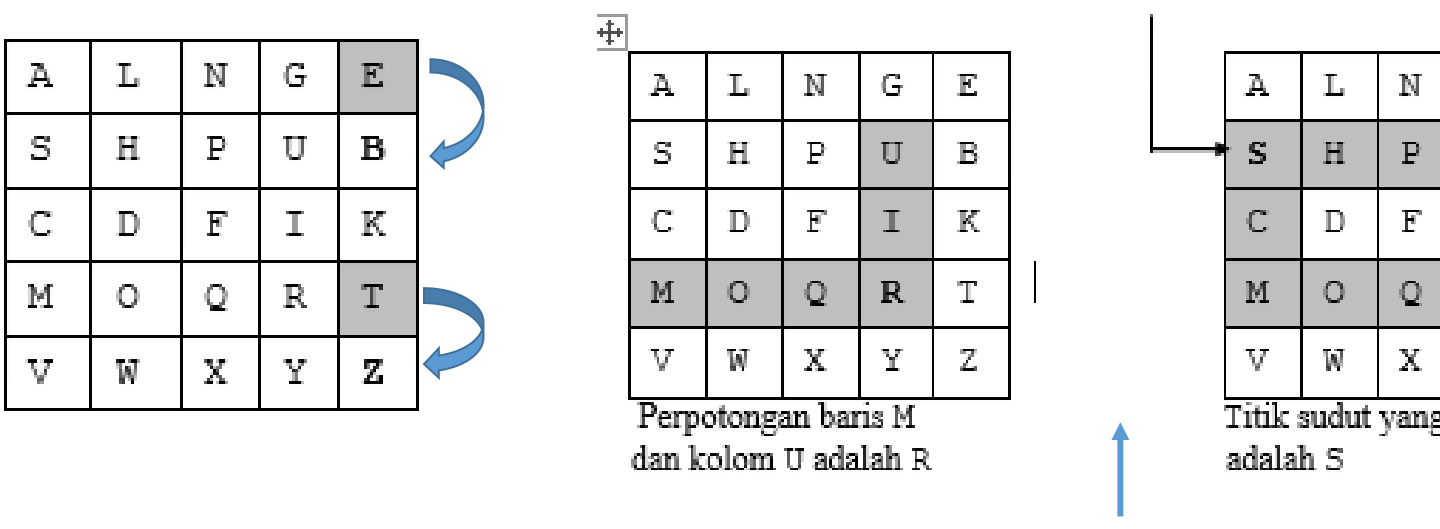
\includegraphics[width=157.50mm,height=145.53mm]{../../images/llm/page_079_img_01.png}%
\end{textblock*}

\end{document}
